\ifx\isEmbedded\undefined

\documentclass[12pt]{report}
\usepackage{tikz}
% FONT RELATED
%\usepackage{times} %Move to times font
\usepackage[labelfont=bf,textfont=it]{caption}

% LINKS, PAGE OF CONTENT, REF AND CROSS-REF, HEADERS/FOOTERS
\usepackage{hyperref}
\usepackage{fancyhdr}



% FIGURES, GRAPHICS, TABLES
%\usepackage{subfig}

%\usepackage{graphicx}
\usepackage{parskip}
%\usepackage{subfigure}
%\usepackage[dvips]{graphicx}
%\usepackage{pgfkeys}% gantt chart
\usepackage{lscape}
\usepackage{rotating}

% Algorithms
%\usepackage[ruled]{algorithm2e}

% COLOURS, TEXT AND FORMATTING
\usepackage{array}
\usepackage{color}
\usepackage{setspace}
\usepackage{longtable}
\usepackage{multirow}

% ADVANCED MATHS, PSEUDO-CODE
\usepackage{amsmath}
\usepackage{amssymb}
\usepackage{alltt}
\usepackage{gensymb}

% GANTT

\usepackage{pgfgantt}

% algorithm
\usepackage{algorithm,algpseudocode}
\usepackage{algorithmicx}

\usepackage{subfig}


\usepackage{adjustbox}

% BIBLIOGRAPHY
\usepackage[authoryear]{natbib}
\bibpunct{[}{]}{;}{a}{}{,}

% USE IN DISSER:

\setlength\oddsidemargin{1.5cm}
\setlength\evensidemargin{5cm}

\setlength\textheight{9.0in}
\setlength\textwidth{5.1in}

% indent at each new paragrapg
\setlength\parindent{0.5cm}

\setlength\topmargin{-0.2in}
\renewcommand{\baselinestretch}{1.3}



%REPORT
\algdef{SE}[DOWHILE]{Do}{doWhile}{\algorithmicdo}[1]{\algorithmicwhile\ #1}%
\newcommand{\HRule}{\rule{\linewidth}{0.0mm}}
\newcommand{\argmin}{\operatornamewithlimits{argmin}}
\newcommand{\argmax}{\operatornamewithlimits{argmax}}
% Color definitions (RGB model)
\definecolor{ms-comment}{rgb}{0.1, 0.4, 0.1}
\definecolor{ms-question}{rgb}{0.4, 0.0, 0.0}
\definecolor{ms-new}{rgb}{0.2, 0.4, 0.8}



\begin{document}
\fi
\chapter{3D shape registration}
\label{chap:mesh}
This chapter presents a novel consistent non-isometric registration approach to handle large deformation and reduce the chance of occurrence of fold-over and intersection. The proposed \emph{consistent} energy only requires a small number of landmarks with little user manual input. It constrains the template in an \textit{as-similar-as-possible} way so that local scales are allowed to change and angles of triangle meshes are as mush as preserved, which enables it to address shapes in large size variation with less shear distortion. Extensive experimental results have demonstrated the effectiveness of CASAP in comparison to the state-of-the-art approaches.

Over the last two decades, \emph{non-rigid registration} has been an active research topic \citep{van2011survey}. \emph{Non-rigid registration} can be generally divided into \emph{isometric} and \emph{non-isometric}. \emph{Isometric registration} aims at finding a set of local rigid transformations but lacks local scalability due to its length-preserving property. \emph{Non-isometric registration} can be further classified into: \emph{equiareal}, \emph{smooth} and \emph{similar}. Specifically, \emph{equiareal registration} has scale-preserving property but is unable to address size difference between the template and the target. In contrast, \emph{smooth registration} based on smoothness regularization afford to size difference. However, it allows piecewise stretching transformation, which can result in shear distortion. \emph{Similar registration} fits the deformation gradient into a similarity matrix, which is an isotropic scale factor times a rotation matrix. The scale factor is able to handle size difference while the rotation matrix part prevents local stretch and distortion. Thus it has been widely used in many applications~\citep{yamazaki2013non,yoshiyasu2014conformal,papazov2011deformable} to align surfaces with different sizes and details. However, the energies they adopt to constrain the local deformation similarity are not \emph{consistent}. This may tend to produce fold-over and self-intersection during transformation.

To our best knowledge, there is no such a surface registration method which takes the local scalability and consistency into consideration at the same time. In this report, we propose a \emph{consistent as-similar-as-possible} (CASAP) surface registration approach. Given a small number of feature points, CASAP is not only able to fit the template to the target with different size and poses, but also preserves the structure of the template well, which is a quite important property in surface cross-parameterization.


\section{CASAP surface registration}
 Given a template surface $\mathcal S$ and a target surface $\mathcal T$, the goal of surface registration is to deform the surface $\mathcal S$ into $ \mathcal S'$ so that $\mathcal{S'}$ can be sufficiently close to surface $\mathcal T$ with structure preserved and less distortion. With that purpose in mind, we enforce \emph{consistent} \emph{as-similar-as-possible} (ASAP) regularization on the template surface when we are attracting it to the target. Let $\mathbf p, \mathbf  p',\mathbf  q$ denote the vertex positions on surface $\mathcal S,\mathcal  S',\mathcal  T$ respectively, we define the cost function as
\begin{equation}
E(\mathbf p') = w_{d}E_{d}(\mathbf p') + w_cE_c(\mathbf p') + w_fE_f(\mathbf p'), \label{energy}
\end{equation}
where $E_{d}$ measures ASAP deformation consistency, $E_c$ penalizes distances between the points of template and their correspondences on the target, and $E_f$ penalizes distances between the feature points of template and target surface. The weights before these energy terms adjust the influence they account for in total energy. As $E_{d}$ has been introduced in last chapter, in the following subsections, we will introduce the last two energy terms.

\subsection{Correspondence  constraints}
In order to attract points on the template towards the target, we need to find their correspondent vertices on the target surface. Many works~\citep{yamazaki2013non,yoshiyasu2014conformal,gilles2010creating} regard the closest points as goal positions, however, correspondences chosen by these approaches are not quite appropriate as they only consider distances between the closest points of template and target surface. Inspired by~\citep{qixing2008non,papazov2011deformable} we will also consider feature descriptors and smooth factor. Starting from the closest points on the target, we then flood over their neighbors to find out the smallest matching energy points until converge. We define matching energy $E_m$ between points of the template and the target as
\begin{equation}
E_m(\mathbf p_i, \mathbf q_j) =\|d_f(\mathbf p_i, \mathbf q_j)-\overline{d_f(\mathbf p_i, \mathbf q_j)}\|^2,
\end{equation}
where $\mathbf p_i$ is vertex $i$ on template surface and $\mathbf q_j$ is vertex $j$ on target surface; the feature descriptors distance is defined as $d_f(\mathbf p_i, \mathbf q_j)=f(\mathbf p_i)-f(\mathbf q_j)$, where $f(v)$ is the feature vector for vertex $v$, we concatenate all feature descriptors into a single feature vector; the mean value distance $\overline{d_f(\mathbf p_i, \mathbf q_j)} = \frac{1}{|\mathcal{N}(j)|+1}\sum_{k \in \mathcal{N}(j)\cup j}d_f(\mathbf p_i, \mathbf q_k)$, where $\mathcal{N}(j)$ is the 1-ring neighbors of vertex $j$ on the target surface. The minimization of $E_m$ will result in a smoother correspondence field than the methods that depend on the descriptor similarity only.

There is a great number of feature descriptors that characterize the geometric properties of the point or of its neighborhood, often in a multi-scale way, for example, various notions of curvature (Gaussian, mean)~\cite{meyer2003discrete}, diffusion-based descriptors, such as the Heat or Wave Kernel Signatures~\cite{sun2009concise,aubry2011wave}, or more classical descriptors such as spin images or shape contexts~\cite{johnson1999using,belongie2002shape}. In our experiment we concatenate vertex position, vertex normal, multi-scale mean curvatures~\cite{panozzo2010efficient}, Wave Kernel Signatures~\cite{aubry2011wave} and Scale-invariant Heat Kernel Signatures~\cite{bronstein2010scale} to form a feature vector.\\

In order to prevent unnecessary matchings, we filter out the pairs if the distance between them exceeds $D$ or if the angle between their normals exceeds a threshold $\Theta$. Thus the algorithm of finding correspondence $\mathbf q_{\text{idx}(i)}$ on the target surface for each point on the template can be summarized as Algorithm \eqref{findcorrespondence}, where $\text{idx}(i)$ is the index of the target point that is matched with template vertex $i$.
\begin{algorithm}[]
\caption{Find correspondence for template vertex $p_i$}
\label{findcorrespondence}
\begin{algorithmic}[1]
    \State Find the closest point $\mathbf q_j$ on the target
    \If{the distance between $\mathbf p_i$ and $\mathbf q_j$ exceeds $D$ \textbf{or} the angle between their normals exceeds $\Theta$}
        \State  \textbf{return} NULL
    \EndIf
    \State $k = j$
    \Do
        \State $j = k$
        \State Find $k \in \mathcal{N}(j)\cup j$ which minimizes $E_m$
    \doWhile{$k \neq j$} % <--- use \doWhile for the "while" at the end
    \State $\text{idx}(i) = k$
    \State  \textbf{return} $\mathbf q_{\text{idx}(i)}$
\end{algorithmic}
\end{algorithm}
After given the correspondence of template vertices, the template surface can be attracted towards the target according to the matching pairs. However, in order to avoid extreme distortion in tangential space, rather than attracting the template points to their correspondences directly, we attract them to the projections of their correspondences on their normals denoted by $Proj(\mathbf q_{\text{idx}(i)})$ (Figure \ref{fig:4}). Now the correspondent constraint energy in~\eqref{energy} can be expressed as
\begin{equation}
E_c(\mathbf p') = \|\mathbf C_c\mathbf p'-Proj(\mathbf D_c\mathbf q)\|_F^2,
\end{equation}
where $\mathbf p', \mathbf q$ are the vertex positions on surface $\mathcal S',\mathcal T$ respectively, and $\mathbf C_c, \mathbf D_c$ are the sparse matrices that define the filtered matching correspondences between $\mathcal  S'$ and $\mathcal T$. Assuming the $m$-th correspondence is $\mathbf p_i$ on $\mathcal S'$ and $\mathbf q_{\text{idx}(i)}$ on $\mathcal T$, then
\[
    \mathbf C_c(m,n)=
\begin{cases}
    1,\!\!\!\! & \text{if } n \!=\! i\\
    0,\!\!\!\! & \text{if } n \!\neq\! i
\end{cases},
    \mathbf D_c(k,n)=
\begin{cases}
    1,\!\!\!\! & \text{if } n \!=\! \text{idx}(i)\\
    0,\!\!\!\! & \text{if } n \!\neq\! \text{idx}(i)
\end{cases},
\]
note that m and k may have different dimensions as the number of vertices between the template and the target are not necessary to be the same.
\begin{figure}[th]
	\begin{center}
			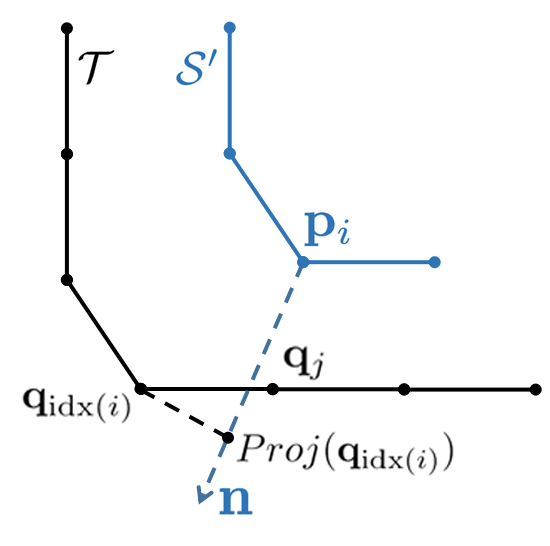
\includegraphics[width=0.6\columnwidth]{./figure/correspondence.png}
	\end{center}
	\caption{$\mathbf q_j$ is the closest vertex on the target to $\mathbf p_i$; $\mathbf q_{\text{idx}(i)}$ is the correspondent vertex found by minimizing the matching energy; $\mathbf{n}$ is the normal vector of $\mathbf p_i$; $Proj(\mathbf q_{\text{idx}(i)})$ is the projection of $\mathbf q_{\text{idx}(i)}$ onto normal vector $\mathbf n$. }
	\label{fig:4}
\end{figure}

\subsection{Feature point constraints}
For the fitting of the template's pose and size to the target, several feature correspondences are required to established. Feature point constrains are designed to drag feature points on the template towards corresponding target ones. This constraint energy can be represented as
\begin{equation}
E_f(\mathbf p') = \|\mathbf C_f \mathbf p' - \mathbf D_f \mathbf q\|_F^2,
\end{equation}
where $\mathbf C_f, \mathbf D_f$ are the sparse matrices that define the feature point pairs between $\mathcal S'$ and $\mathcal T$.


\subsection{Optimization}
In this subsection, we introduce the optimization algorithm to minimize the total energy in \eqref{energy}. There are two loops in the optimization: the outer loop searches for the correspondent vertices to construct $E_c$, the inner loop optimizes the deformed vertex positions by minimizing $E(\mathbf p')$. Once the inner loop is converged, weights are adjusted and a new outer iteration starts again.

Taking derivative of the total enery \eqref{energy} w.r.t. $\mathbf p'$ gives us a linear system:
\begin{equation}
\mathbf A^T\mathbf A\mathbf p' = \mathbf A^T\mathbf b,\label{linear}
\end{equation}
where
\begin{align*}
\mathbf A =\begin{pmatrix}w_{d}\mathbf L\\w_c\mathbf C_c\\w_f\mathbf C_f\end{pmatrix}, \mathbf b = \begin{pmatrix}w_{d}\mathbf d\\w_cProj(\mathbf D_c \mathbf q)\\w_f\mathbf D_f \vec q\end{pmatrix},
\end{align*}
where $\mathbf L$ and $\mathbf d$ from equation \eqref{DeformationLinearSystem}.

Up to now, the routine of \emph{consistent} ASAP surface registration can be summarised as Algorithm \eqref{casapsurfaceregistration}.
\begin{algorithm}[]
\caption{\emph{Consistent} ASAP Surface registration}
\label{casapsurfaceregistration}
\begin{algorithmic}[1]
    \State Specify the feature points.
    \While{not converged}
        \While{not converged}
            \State Compute $\mathbf R_i$ by solving equations \eqref{R}.
            \State Compute $s_i$ by solving equations \eqref{s}.
            \State Compute $\mathbf p'$ and update surface $\mathcal S'$ by solving equation \eqref{linear}.
        \EndWhile
        \State Adjust weights in \eqref{linear} and construct $E_c$
    \EndWhile
\end{algorithmic}
\end{algorithm}

\section{Coarse-to-fine fitting strategy}
To improve the efficiency and robustness of registration, we take a coarse-to-fine fitting strategy. Instead of fitting overall template surface from the beginning, a coarse mesh is extracted from the original template mesh and then fitted to several feature points from the target model to roughly adjust the overall size of the template. In this way, approximated goal positions are obtained which is a better initial guess of fine fitting leading to fast converge and it also reduces the fold-over occurrence. Afterwards, a dense mesh is rebuilt from the deformed coarse mesh and fine fitting step is performed to produce the final result.
 \begin{figure*}[!hptb]
 \centering

 \captionsetup[subfigure]{labelformat=empty}
 \centering

			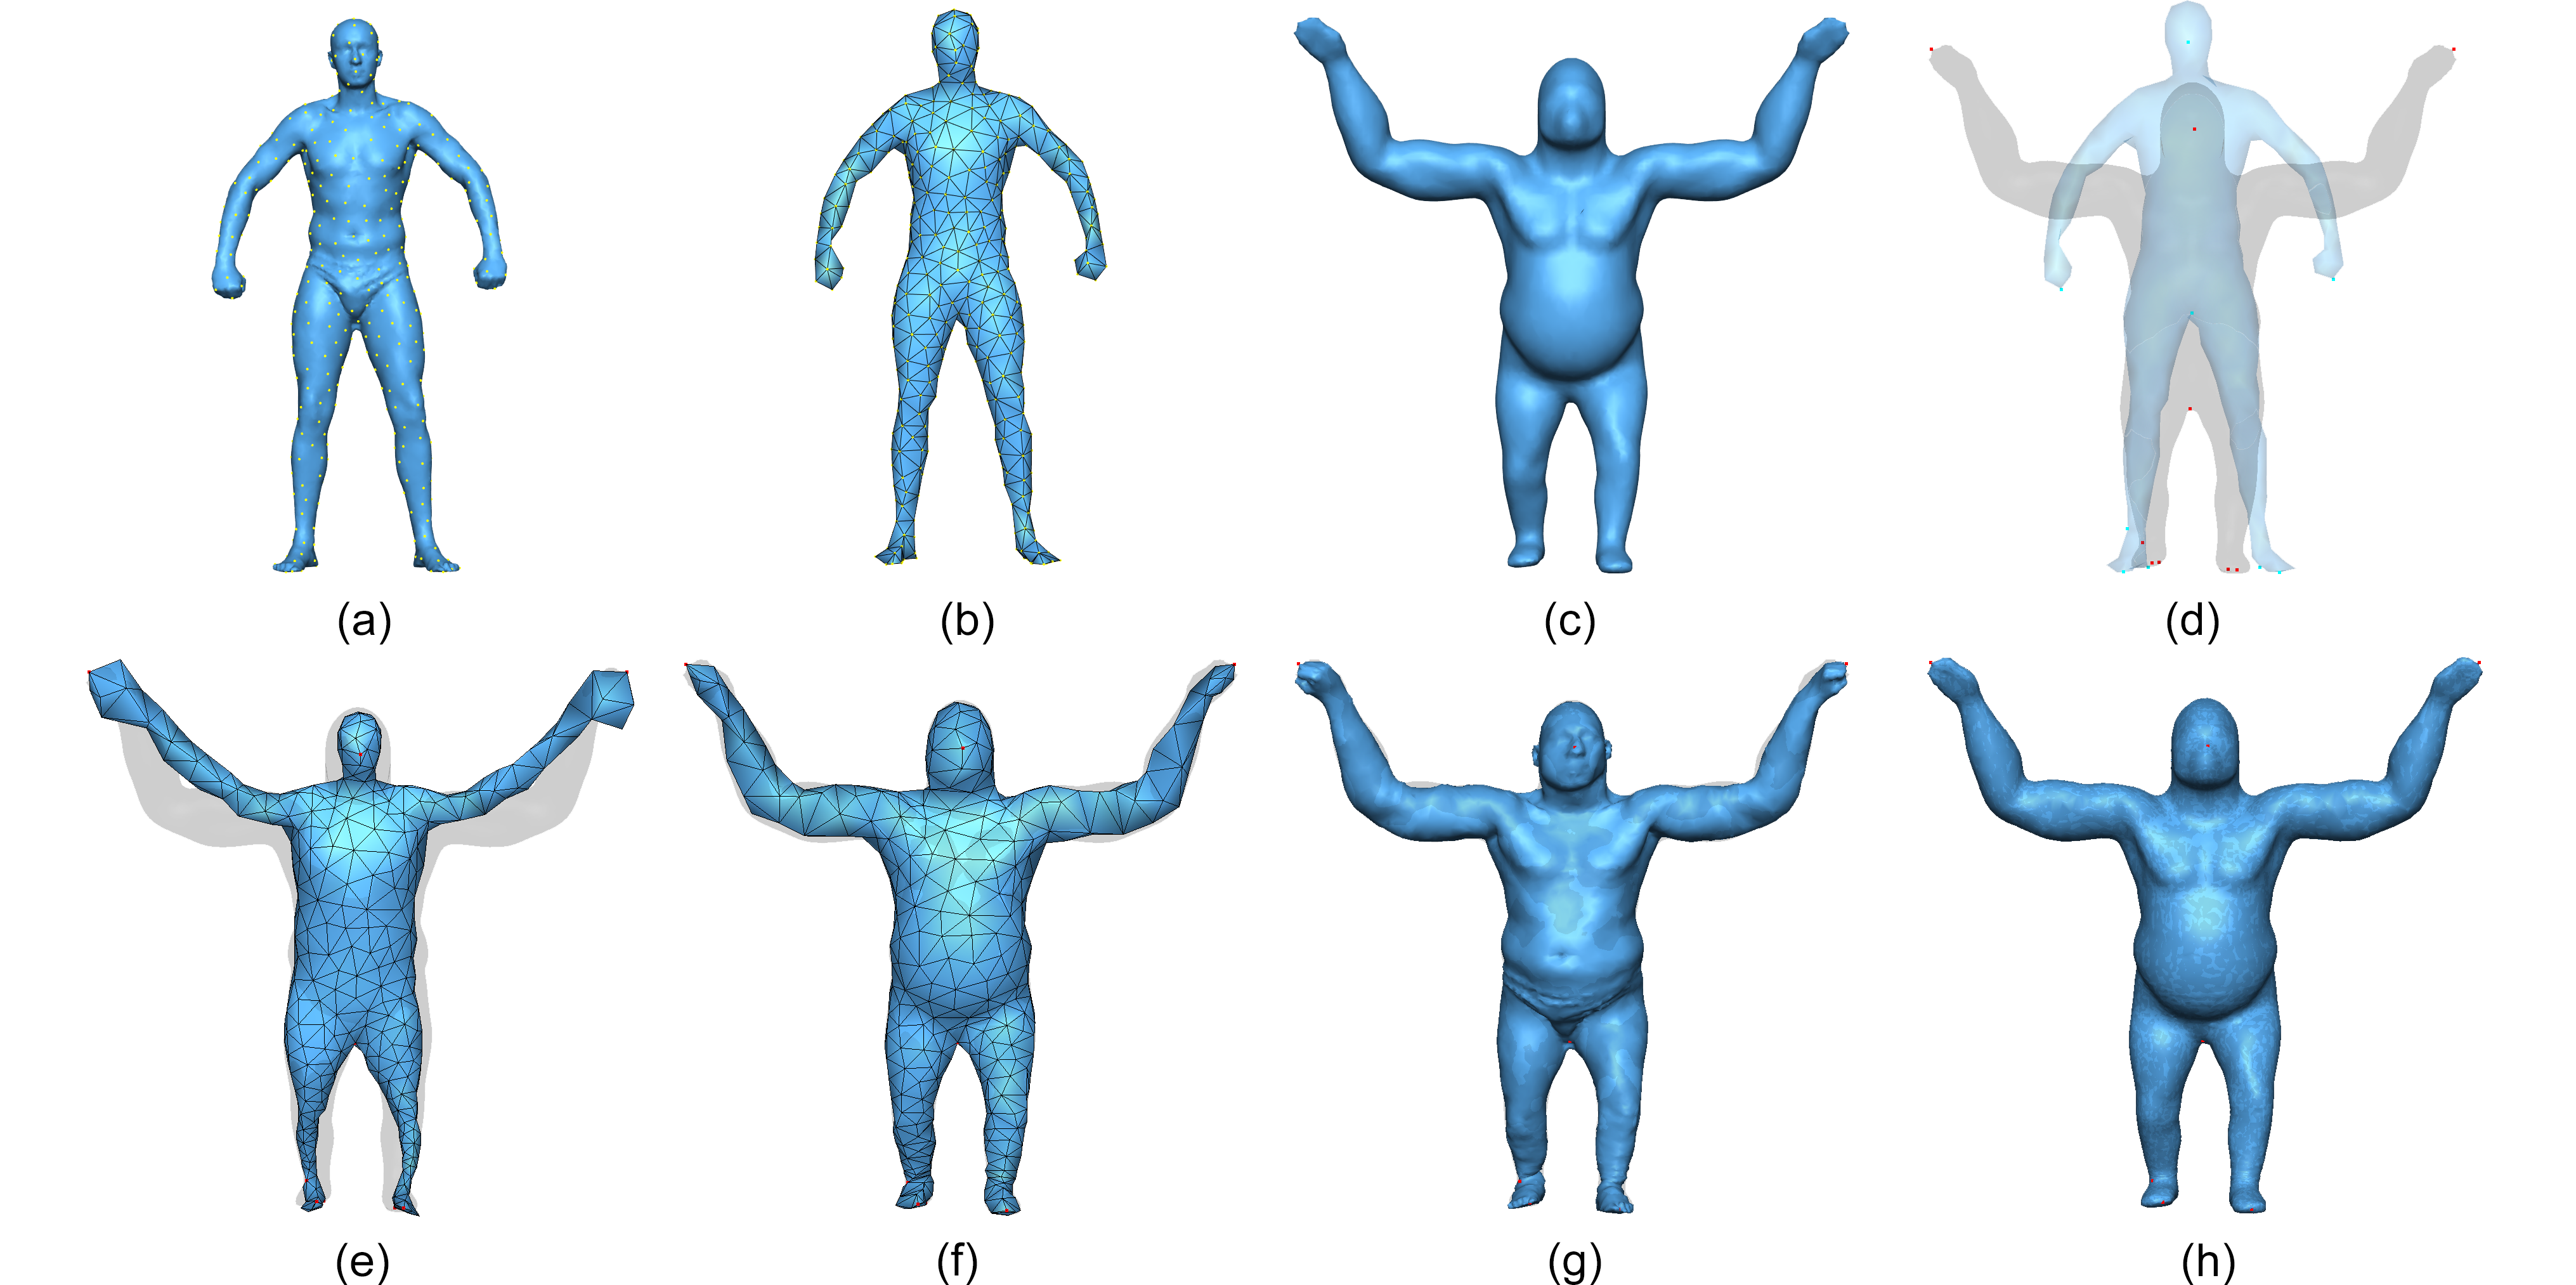
\includegraphics[width=\textwidth]{./figure/overview.png}


     \caption{Surface registration algorithm overview: (a) 500 sampled points (marked as yellow dots) from 12500 vertices of the original template model via farthest point sampling technique; (b) Remeshing from the sampled points as embedded coarse mesh; (c) Input of target surface; (d) The feature points specified by users (red dots for target and cyan dots for template); (e) Coarse fitting; (f) Mid-scale fitting; (g) Reconstructed through embedded deformation; (h) Fine fitting.}
     \label{fig:overview}
 \end{figure*}
\subsection{Fitting Steps}
There are four fitting steps: initialization, coarse fitting, mid-scale fitting and fine fitting:\\

$\textbf{Initialization}$ ~~In this step, a coarse mesh is extracted from the template first. We employ the farthest point sampling approach~\citep{moenning2003fast} to sample certain number of vertices to represent the shape of objects approximately (Figure \ref{fig:overview}a). Note that all of the sampled vertices are the subset of the original vertex set. Then the geodesic remeshing technique~\citep{surazhsky2005fast} is used to generate the coarse mesh from the sampled points (Figure \ref{fig:overview}b). \\

$\textbf{Coarse}$ $\textbf{ Fitting}$ ~~We utilize the similarity constraints and feature point constraints to fit the coarse mesh to the feature points on the target so that the size and post of the template are roughly adjusted to the target (Figure \ref{fig:overview}e).\\

$\textbf{Mid-scale}$ $\textbf{ Fitting}$ ~~After fitting the template roughly to the target using feature points, the coarse mesh is deformed gradually toward the target. Apart from the two kinds of constraints adopted in the first step, correspondence constraints are also applied to achieve template attraction (Figure \ref{fig:overview}f).\\

$\textbf{Fine}$ $\textbf{ Fitting}$ ~~In this stage, a dense mesh is reconstructed from the deformed coarse mesh by embedded deformation~\citep{sumner2007embedded} (Figure \ref{fig:overview}g). The extracted coarse mesh is considered as deformation graph laid under the the dense mesh. From formulas \eqref{s} and \eqref{R}, we associate an affine transformation with each vertex in the coarse graph. The deformed positions of vertices in the dense mesh can be calculated from the transformations of the deformation graph. We use the same approach as~\cite{yoshiyasu2014conformal} to rebuild the dense mesh. Again, all the constraints are performed to fit the dense mesh to the target (Figure \ref{fig:overview}h).


\subsection{Weights and parameters}
In the initialization step, we regard the feature point constraints as boundary condition to induce deformation. In next two steps, we set $D = 0.02r_{box}$ and $\Theta = 90^\circ$ in our examples, where $r_{box}$ is the length of the bounding box diagonal. As for the weights in the linear system \eqref{linear}, we use $w_{d} = 1000$, $w_{c} = 5$, $w_{f} = 10^5$ in the coarse fitting stage and divide $w_{d}$ by $1.1$ after every iteration until it less than $1$. In the fine fitting, we take the same procedure with $w_f = 1$.



\section{Experiments and Results}
We tested our algorithm on various surfaces. For surface deformation, the data (cylinder and bar) in ~\citep{botsch2008linear} are adopted. We show twist and translation deformation on these meshes in Figure \ref{fig:deformation_comparison}. For surface registration, we use the human head mesh, 3D face scanning, the human body and animal models which are from SCAPE, TOSCA data sets. All the algorithms are implemented in MATLAB and all the statistics are measured on an Intel Xeon E5 3.4 GHz 64-bit workstation with 16GB of RAM. \\

$\textbf{Generic models}$ ~~We apply CASAP registration technique to register from one human head with holes to a face scanning from another human (Figure \ref{fig:1}); from a human body to a gorilla (Figure \ref{fig:1}, \ref{fig:overview}); from a pig to a horse (Figure \ref{fig:registration_comparison}). Each pair has large difference on size or details. CASAP not only is able to handle size difference as shown in whole-body registration example in Figure \ref{fig:overview}, but also can capture geometrical details such as the human expression (Figure \ref{fig:1}) and preserve the structure of the template well, thus reducing the risk of producing fold-over (Figure \ref{fig:1}, \ref{fig:registration_comparison}).\\

\begin{figure}[ht]
\begin{center}
\includegraphics[width=\columnwidth]{./figure/figure1.png}
\end{center}
\caption{\emph{Consistent as-similar-as-possible} (CASAP) non-isometric registration. Given a small number of feature correspondences (seven for the head registration and nine for the whole-body registration) only, CASAP not only is capable of fitting the template towards the target with different size (revealed in the whole-body registration example), but also captures the details well (shown in the face registration example) and preserves the structure of the template (seen from the colored wireframe shading mode).}
\label{fig:1}
\end{figure}

$\textbf{Comparisons}$ We compare our registration technique to other state-of-the-art algorithms: \emph{as-conformal-as-possible} surface registration (ACAP)~\citep{yoshiyasu2014conformal}, similarity-invariant shape registration (ASAP)~\citep{yamazaki2013non}, the embedded deformation technique (ED)~\citep{sumner2007embedded}, the shape matching based registration technique that minimizes the \emph{as-similar-as-possible} energy (SM-ASAP)~\citep{papazov2011deformable}, the Laplacian surface editing technique (LSE)~\citep{sorkine2004laplacian} and the registration technique that utilizes the point-based deformation smoothness regularization (PDS)~\citep{amberg2007optimal} in Figure \ref{fig:registration_comparison}. ACAP employs nonlinear conformal stiffness and regularization terms in registration process, which produces the closest results to CASAP. However, since the regularization energy it adopts is not \emph{consistent}, fold-overs still occur around the left wrist of gorilla and the neck of horse. ASAP and SM-ASAP do not require specifying feature points, but they are only able to handle surfaces with close initial alignment and similar poses. ED is an isometric counterpart of ACAP. As it cannot adjust local scale, ED may produce poor initial shape estimation, which makes parts of surface converge to inaccurate places as shown at the right leg of gorilla. LSE cannot handle large deformation as it use a linear approximation of similar transformation. PDS is based on smoothness regularization, but it is too weak to handle shear distortions. Only CASAP exhibits no fold-over and almost no distortion in the examples, which produce quite pleasant visual results.
 \begin{figure*}[!thpb]
 \begin{adjustbox}{addcode={\begin{minipage}{\width}}{\caption{%
     Different surface registration methods comparison. The left two columns are inputs while the rest are outputs by different surface registration methods. The yellow and red dots indicate the feature points on the template and the target respectively. The corresponding points are with same colors. \label{fig:registration_comparison}
      }\end{minipage}},rotate=90,center}
        \includegraphics[scale=0.06]{./figure/registration_comparison.png}
 \end{adjustbox}
 \end{figure*}



% \begin{figure*}[!thpb]
% \centering
%
% \captionsetup[subfigure]{labelformat=empty}
% \centering
%
%			\includegraphics[scale=0.06,angle=90]{./figure/registration_comparison.png}
%
%     \caption{Different surface registration methods comparison. The left two columns are inputs while the rest are outputs by different surface registration methods. The yellow and red dots indicate the feature points on the template and the target respectively. The corresponding points are with same colors.}
%     \label{fig:registration_comparison}
% \end{figure*}
\begin{figure}[!h]
\centering
 \subfloat[]{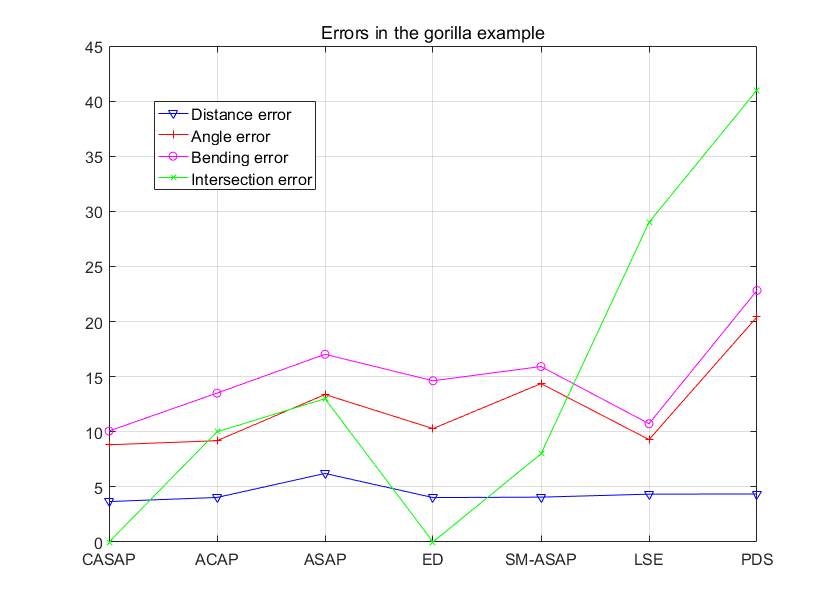
\includegraphics[width=0.5\textwidth]{./figure/gorilla_error.png}\label{fig:gorilla_error}}
 \subfloat[]{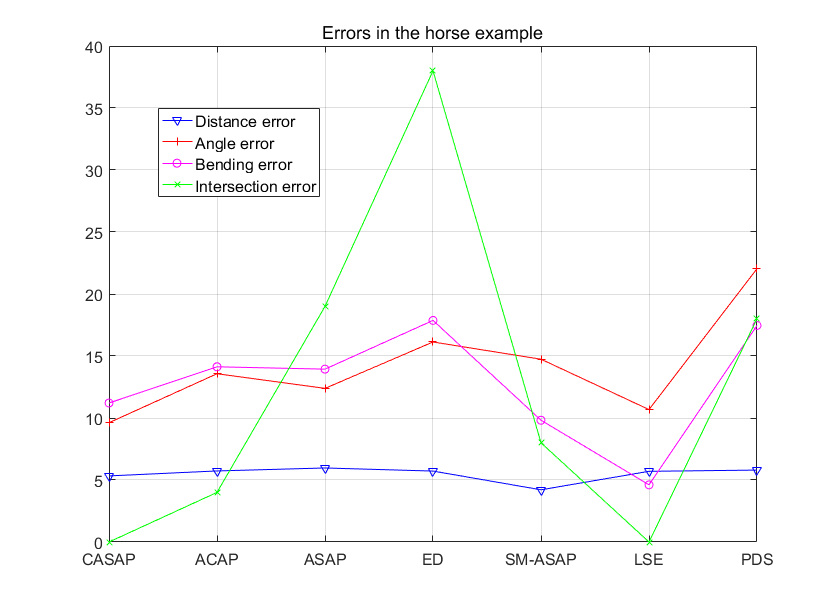
\includegraphics[width=0.5\textwidth]{./figure/horse_error.png}\label{fig:horse_error}}
 \caption{Quantitative comparison for the gorilla and horse registration results respectively.}
 \label{fig:errors}
\end{figure}




% \begin{table*}[!hptb]
%%\hspace{-20in}
% \caption{Quantitative comparisons, D, A, B and I indicate distance error[\%], angle error [$^\circ$], bending error[$^\circ$] and intersection error respectively.\label{tbl:comparison}}
%\resizebox{\textwidth}{!}{
%  \centering
%  \begin{tabular}{  c | c | c | c | c | c | c | c | c | c | c | c | c | c | c | c | c | c | c | c | c | c | c | c | c | c | c | c | c  }
%    \hline
%     & \multicolumn{4}{c|}{CASAP}& \multicolumn{4}{c|}{ACAP} &\multicolumn{4}{c|}{ASAP} & \multicolumn{4}{c|}{ED}& \multicolumn{4}{c|}{SM-ASAP} &\multicolumn{4}{c|}{LSE} &\multicolumn{4}{c}{PDS} \\ \hline
%     & D & A & B & I & D & A & B & I & D & A & B & I & D & A & B & I & D & A & B & I & D & A & B & I & D & A & B & I \\ \hline
%     %Head & 0.25 & 10.7 & 14.3& 0 & 0 & 0 & 0 &0 &0 &0 & 0.31 & 12.3 & 15.9 & 0.31 & 11.9 & 20.4 & 0.26 & 11.8 & 21.1 & 4.76 & 11.5 & 17.2 & 3.23 & 13.8 & 23.6 & 3.23 & 13.8 & 23.6 \\ \hline
%     Gorilla & \textbf{3.67} & \textbf{8.82} & \textbf{10.07} & \textbf{0} & 4.04 & 9.19 &13.51 & 10 & 5.22 & 13.38 & 17.03 & 13 & 4.03 & 10.29 & 14.63 & 0 & 4.07 & 14.37 & 15.92 & 8 & 4.34 & 9.29 & 10.73 & 29 & 4.36  & 20.42 & 22.82 & 41\\ \hline
%     Horse & \textbf{5.33} & \textbf{9.62} & 11.21 & \textbf{0} & 5.73 & 13.57 & 14.13 & 4 & 5.97 & 12.39 &13.94 & 19 & 5.72 & 16.13 & 17.87 & 38 & 4.21 & 14.74 & 9.82 & 8 & 5.70 & 10.68 & \textbf{4.61} & 0 & 5.80 & 22.04 & 17.46 & 18\\ \hline
%  \end{tabular}
%}
% \end{table*}

 \begin{table*}[!hptb]
%\hspace{-20in}
 \caption{Iteration steps and timings (in seconds). \#O, \#I indicate the number of outer iteration steps and total inner iteration steps respectively. ``Inner'' indicate the average time required for each inner iteration step. ``Total'' indicate the total registration time.\label{tbl:timing}}
\resizebox{\textwidth}{!}{
  \centering
  \begin{tabular}{  c | c | c | c | c | c | c | c | c | c | c | c | c | c | c | c | c | c | c | c | c | c | c | c | c | c | c | c | c  }
    \hline
     & \multicolumn{4}{c|}{CASAP}& \multicolumn{4}{c|}{ACAP} &\multicolumn{4}{c|}{ASAP} & \multicolumn{4}{c|}{ED}& \multicolumn{4}{c|}{SM-ASAP} &\multicolumn{4}{c|}{LSE} &\multicolumn{4}{c}{PDS} \\ \hline
     & \#O & \#I & Inner & Total & \#O & \#I & Inner & Total & \#O & \#I & Inner & Total & \#O & \#I & Inner & Total & \#O & \#I & Inner & Total & \#O & \#I & Inner & Total & \#O & \#I & Inner & Total \\ \hline
     %Head & 0.25 & 10.7 & 14.3& 0 & 0 & 0 & 0 &0 &0 &0 & 0.31 & 12.3 & 15.9 & 0.31 & 11.9 & 20.4 & 0.26 & 11.8 & 21.1 & 4.76 & 11.5 & 17.2 & 3.23 & 13.8 & 23.6 & 3.23 & 13.8 & 23.6 \\ \hline
     Gorilla & 54 & 2882 & \textbf{0.035} & 100.87 & 73 & 313 & 0.338 & 105.94 & 20 & 683 & 0.038 & 25.95 & 10 & 1547 & 0.379 & 586.91 & 9 & 50 & 0.376 & 18.783 & \textbf{1} & \textbf{1} & 0.357 & \textbf{0.357} & 500  & 2166 & 0.036 & 77.976\\ \hline
     Horse   & 54 & 2915 & \textbf{0.032} & 93.28  & 73 & 276 &0.423 & 116.62 & 20 & 1501 & 0.033 & 49.53 & 10 & 1597 & 0.508 & 811.95 & 9 & 48 & 0.355 & 17.025 & \textbf{1} & \textbf{1} & 0.371 & \textbf{0.371} & 500 & 1870 & 0.035 & 65.45\\ \hline
  \end{tabular}
}

 \end{table*}


From the perspective of quantitative evaluation,  following the same criterion as in \citep{yoshiyasu2014conformal}, we measure 1) distance error, which is the average distance from the vertices of the deformed template to the corresponding points of the target relative to the bounding box diagonal, 2) angle error, which is the average angle deviation from the template, 3) bending error, which is the average deviation in dihedral angles from the template, 4) intersection error, which is the number of self-intersecting faces. These statistics can be found in Figure \ref{fig:errors}. All the errors of CASAP are the smallest among all the techniques except the bending error in horse example, in which the error of LSE is least. However, the registration result of LSE is not desirable due to its disability of handling large rotations. The number of self-intersecting faces in CASAP is zero, which reveals the ability of CASAP to reduce the change of fold-over and shear distortion appearance.

The number of iteration steps and timings are shown in Table~\ref{tbl:timing}. The time required for a single inner iteration of CASAP is minimum. Although it requires more iteration steps than ACAP to converge, the total registration time it spends is less than ACAP.

%$\textbf{Number of feature points required}$ ~~ Previous methods \cite{sumner2004deformation,yeh2011template} require specifying 20-70 feature points, whereas our technique requires less than 20 points: 7 for the face registration (Figure \ref{fig:1}), 9 for the whole-body registration(Figure \ref{fig:1}, \ref{fig:overview}), 15 for registration from pig to horse (Figure \ref{fig:registration_comparison})). That is because CASAP provides a good initial shape approximation, and the \emph{consistent} energy preserves the template structure and angles well.


\section{Conclusion}
We have presented a novel surface registration approach (CASAP) that constrains deformations locally as similar as possible. With the proposed \emph{consistent} regularization energy, CASAP not only results in \emph{consistent} discretization for surface, but also requires a small number of landmarks with only little user effort. Besides, CASAP is constrained in an as-similar-as-possible way so that angles of triangle meshes are well preserved and local scales are allowed to change. Experiments have shown that CASAP produced more accurate fitting results and preserved angles better than previous methods.



\ifx\isEmbedded\undefined
% References
\addcontentsline{toc}{chapter}{References}
\pagebreak
\end{document}
\fi
